\documentclass[12pt]{article}
\usepackage{makeidx}
\usepackage[margin=1in]{geometry}  % set the margins to 1in on all sides
\usepackage{graphicx}              % to include figures
\usepackage{amsmath}               % great math stuff
\usepackage{amsfonts}              % for blackboard bold, etc
\usepackage{amsthm}                % better theorem environments
\usepackage{makeidx}               % index
\usepackage[utf8]{inputenc}        % now we have tildes!
\usepackage{wrapfig}               % images
\usepackage{listings}              % Unordered lists
\usepackage{hyperref}              % hyperlinks
\usepackage{xcolor}                % to colorize font
\usepackage{blindtext}             % to colorize font

% Color definitions
\definecolor{landanimal}{rgb}{.545,.1,.1}
\colorlet{ocean}{blue!60!black}
\newcommand{\earth}[1]{\textcolor{landanimal}{#1}}
\newcommand{\water}[1]{\textcolor{ocean}{#1}}

\makeindex

\begin{document}

\begin{titlepage}

\newcommand{\HRule}{\rule{\linewidth}{0.5mm}} % Defines a new command for the horizontal lines, change thickness here

\center % Center everything on the page

%----------------------------------------------------------------------------------------
%	HEADING SECTIONS
%----------------------------------------------------------------------------------------

\textsc{\LARGE Universidad Carlos III de Madrid}\\[1.5cm] % Name of your university/college
\textsc{\Large Aprendizaje Automático}\\[0.5cm] % Major heading such as course name
\textsc{\large Computer Science Engineering}\\[0.5cm] % Minor heading such as course title

%----------------------------------------------------------------------------------------
%	TITLE SECTION
%----------------------------------------------------------------------------------------

\HRule \\[0.4cm]
{ \huge \bfseries Práctica 1: Clasificación y Predicción}\\[0.4cm] % Title of your document
\HRule \\[1.5cm]

%----------------------------------------------------------------------------------------
%	AUTHOR SECTION
%----------------------------------------------------------------------------------------


% If you don't want a supervisor, uncomment the two lines below and remove the section above
\emph{Authors:}\\
Daniel \textsc{Medina García}\\ % Your name
Alejandro \textsc{Rodríguez Salamanca}\\[3cm] % Your name

%----------------------------------------------------------------------------------------
%	DATE SECTION
%----------------------------------------------------------------------------------------

{\large \today}\\[3cm] % Date, change the \today to a set date if you want to be precise

%----------------------------------------------------------------------------------------
%	LOGO SECTION
%----------------------------------------------------------------------------------------

%
\includegraphics{Logo}\\[1cm] % Include a department/university logo - this will require the graphicx package

%----------------------------------------------------------------------------------------

\vfill % Fill the rest of the page with whitespace

\end{titlepage}

\tableofcontents

\newpage
\section*{Introducción}

En esta primera práctica, el equipo de trabajo emplea los conocimientos adquiridos en los anteriores \emph{Tutoriales} para implementar un agente automático que utiliza técnicas de aprendizaje automático para su funcionamiento. Vistas las restricciones que causaba no poder utilizar estas técnicas en el \emph{Tutorial 1}, es ahora el momento de probar si realmente suponen una ventaja o no a la hora de implementar un agente automático para el famoso PacMan. ¿Merece la pena el uso de estas técnicas para este juego? ¿Qué datos son de utilidad y cuáles no para implementar un agente que trabaje con aprendizaje automático? ¿Cómo nos ayuda tratar de predecir las futuras jugadas a la hora de elegir nuestro movimiento? Estas y otras preguntas serán contestadas en la memoria que está a punto de leer.

\newpage
\section{Fase 1: Instancias de Entrenamiento y Test}

Para extraer los datos del juego, se partió de la función utilizada en el tutorial anterior. Esa base fue ampliada con experimentación, añadiendo y quitando atributos según mejoraba o empeoraba el éxito de clasificación del árbol resultante con distintos algoritmos, como será explicado en la \emph{Fase 2}.

Además de los datos que se tienen en la propia jugada, también se han incluido datos futuros en las instancias del fichero \texttt{.arff}. Para implementar esta funcionalidad, se ha utilizado un método de escritura retardada. Así, no se escribe una nueva línea en el fichero hasta que no se conocen todos los datos que se han de escribir, almacenando mientras tanto los datos intermedios. Esto se hizo creando listas globales, que almacenan las líneas incompletas (a falta de datos futuros) en \texttt{future\_lines} y las puntuaciones (para completar las líneas anteriores cuando llegue su turno) en \texttt{future\_score}. Cuando la primera línea esté completa (en este caso, en el sexto turno), se imprimirán en el archivo los datos que ya se tenían junto a los recién llegados, creando así una línea completa.

\newpage
\section{Fase 2: Clasificación}

\subsection{Transformación de datos}

Es este el factor donde el razonamiento sobre los datos puede dar lugar a más variantes. Ya que anteriormente no se han comentado, mencionamos aquí la base de atributos de los que partimos:
\begin{itemize}
    \item \texttt{score} : puntuación actual de PacMan.
    \item \texttt{ghost<N>-living} : True si el fantasma \textless N\textgreater\ sigue vivo, False si ya ha sido comido.
    \item \texttt{distance-ghost<N>} : Distancia ruidosa de PacMan al fantasma \textless N\textgreater.
    \item \texttt{posX} y \texttt{posY} : Coordenadas de PacMan sobre el tablero.
    \item \texttt{direction} : Hacia dónde mira PacMan (último movimiento realizado).
    \item \texttt{wall-<direction>} : True si hay un muro en \textless direction\textgreater, False si vía libre.
    \item \texttt{move} : Movimiento tomado, es la \textbf{clase}.
\end{itemize}

La experimentación ha sido la protagonista en esta fase. Lamentablemente, su protagonismo se ha debido a la búsqueda de nuevas alternativas ante las numerosas pruebas descartadas por ausencia de resultados positivos, como son explicadas a continuación.

\vspace{0.2cm}

Tratamos de agregar los datos que teníamos de forma que resultasen en algún campo que fuese útil para el modelo, y para ello probamos convirtiendo los atributos \texttt{ghost<N>-living} en uno sólo que fuese la suma de los fantasmas vivos (aplicando primero el filtro \emph{NominalToBinary} sobre los cuatro atributos, y luego el filtro \emph{AddExpression} sumándolos todos), obteniendo un decremento de éxito de clasificación de entre el 2.3\% y el 3\%, dependiendo del método utilizado para la evaluación.

Consideramos también la generalización de nuestro agente a un número $N$ de fantasmas. El agente base es válido sólo para partidas con 4 fantasmas, si bien el juego real puede constar de un número distinto de ellos. Para solucionar el problema de jugar con más de cuatro fantasmas, se podrían considerar siempre los 4 fantasmas más cercanos (i.e. los ``mejores''). Pero, ¿y si fueran menos? Podríamos reducir ese 4 hasta 1, de forma que sólo se tuviese en cuenta el fantasma más cercano y el agente siempre fuese a por él obviando a los demás. Si vemos hacia dónde nos está llevando esta línea, observamos que estamos sobredirigiendo el aprendizaje y acabamos imitando al agente del \emph{Tutorial 1}. Por ello, abandonamos estas hipótesis dado que consideramos se alejan de los objetivos de la práctica.

\newpage
\subsection{Experimentación y comparaciones}

En esta fase el equipo dedicó su esfuerzo a realizar tantas pruebas como fuesen posibles, probando diferentes combinaciones de algoritmos, filtros y atributos para generar el modelo basándonos en conocimiento y razonamientos \emph{a priori}.

Para crear un modelo exitoso, hay que tener en cuenta varios factores, a continuación analizaremos cada uno de ellos:

\subsubsection{Elección de los datos de entrada para la creación del modelo}

Para la elección de la entrada para el algoritmo, partimos de dos bases: los datos de ejecución del agente automático (que, para jugar, se informa tan sólo de los sensores que le indican las distancias a cada uno de los fantasmas) y los de las partidas que jugamos los miembros del equipo, viendo los fantasmas. No es difícil llegar a la conclusión de que el agente humano gana las partidas mucho más rápido que el agente implementado en el \emph{Tutorial 1}, pero eso no tenía por qué indicar que necesariamente los datos del agente de teclado generasen un modelo con un mayor éxito de clasificación. Sin embargo, con posteriores pruebas encontramos un aplastante 10-15\% de diferencia en éxito de clasificación a favor del agente de teclado entre los modelos generados para ambos archivos con \emph{J48} y \emph{BFTree} y evaluados con cross-validation, dos de los algoritmos que conocíamos de tutoriales anteriores y sabíamos generaban árboles bastante buenos. La siguiente tabla ilustra los resultados obtenidos:

\begin{center} 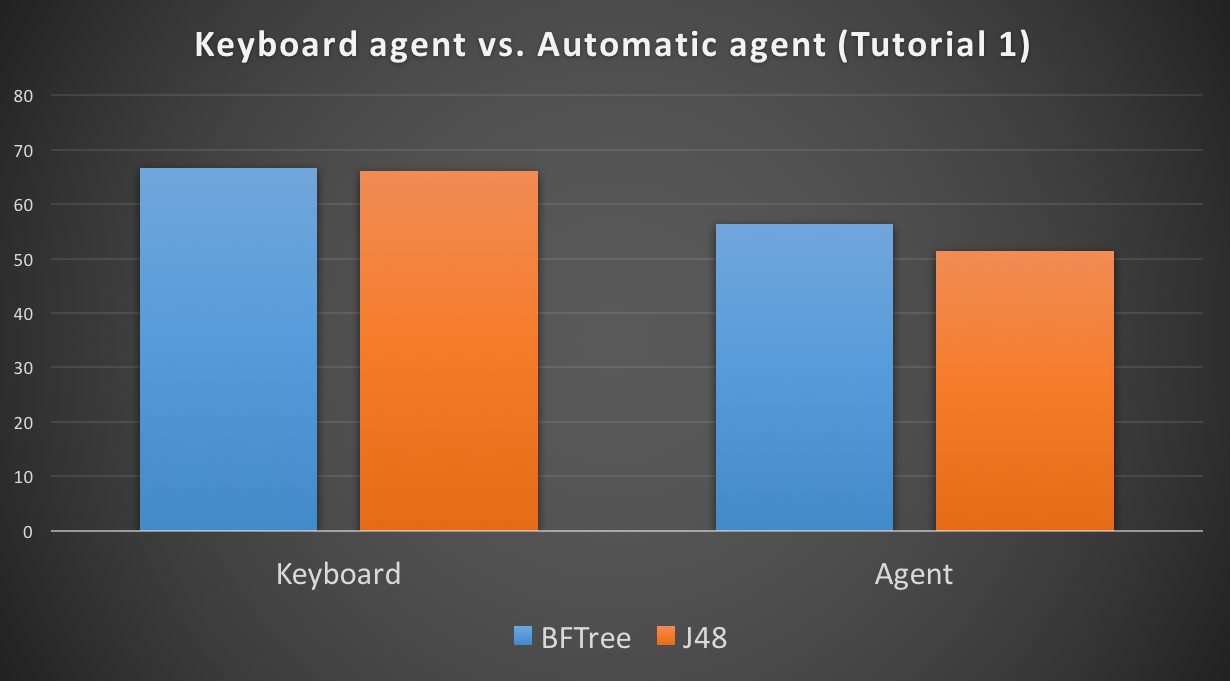
\includegraphics[width=12cm]{kb_vs_aa} \end{center}

Viendo estos datos, nos decantamos por \texttt{training\_keyboard\_edited.arff}, que es el fichero que contiene los datos legales (sin los datos de puntuaciones futuras), para generar el modelo en \emph{Weka}.

\subsubsection{Elección del algoritmo generador de nuestro modelo}

Una vez escogido el archivo que se usará para generar el modelo, comenzamos la comparación entre algoritmos para realizar dicha tarea. Para ello, comparamos varios algoritmos de creación de árboles de decisión evaluándolos tanto con validación cruzada como con dos sets de instancias generadas en partidas jugadas, uno en los mismos mapas que en el entrenamiento y otro en mapas distintos. El éxito de clasificación de cada uno de los algoritmos utilizados se muestra en la siguiente tabla:

\vspace{0.3cm}

\noindent 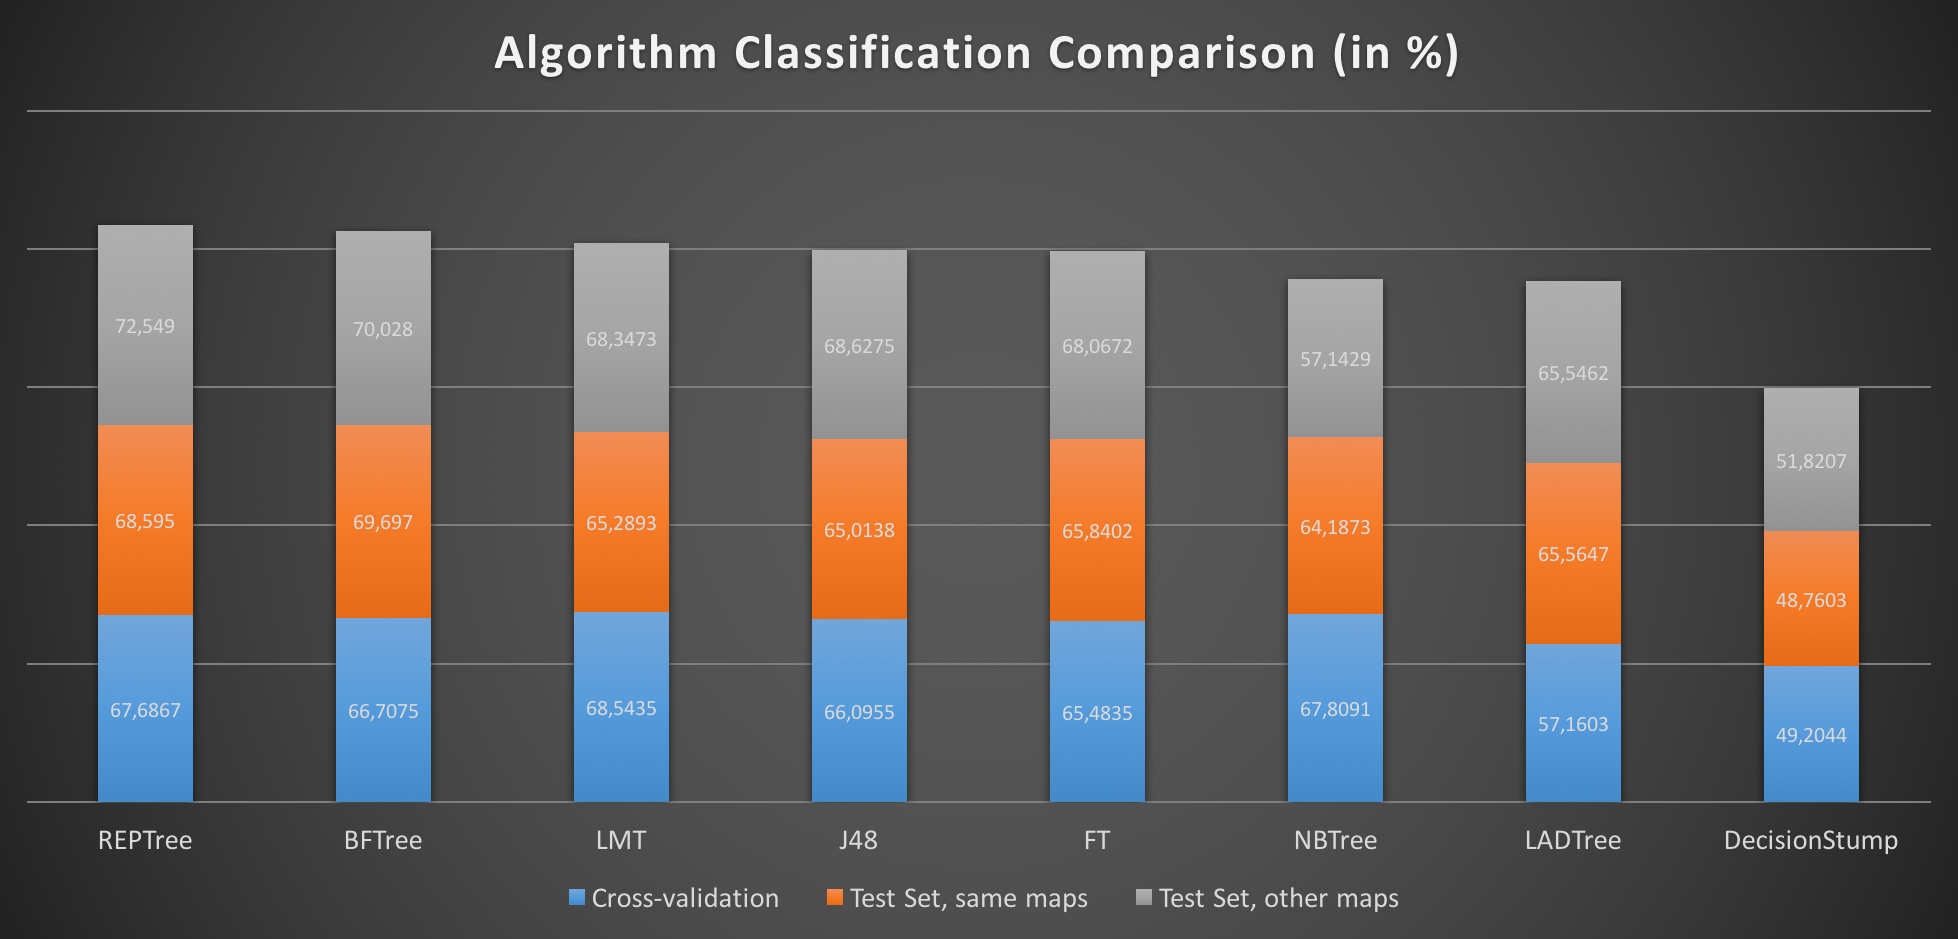
\includegraphics[width=\textwidth]{algorithm_comparison}

\vspace{0.3cm}

Nos sorprendieron los resultados de \emph{REPTree}, un algoritmo que no habíamos utilizado con anterioridad y, sin embargo, obtuvo los mejores resultados. Si bien este algoritmo suele utilizarse para clasificaciones multi-clase, esto no le impide funcionar para una sola clase también, y queda demostrado que con efectividad. Esta información se tendrá muy en cuenta a la hora de elegir el algoritmo generador del modelo en el cual se basará nuestro nuevo agente automático para tomar las decisiones pertinentes, y nos sirve para descartar algunos algoritmos, agilizando los cómputos posteriores.

\subsubsection{Aplicación de filtros para mejorar el comportamiento de los algoritmos}

Intentamos extraer el máximo de información de los datos que ya teníamos, sesgándolos mediante la aplicación de filtros que pudiesen acarrear un mejor funcionamiento de los algoritmos de prueba.

Como el movimiento \texttt{STOP} no aporta valor al juego (no conseguirá acercarse a ningún fantasma), editamos nuestro fichero de datos eliminando las instancias que hubiesen realizado ese movimiento (i.e. aquellas transcurridas entre que empieza el juego y el jugador de teclado pulsa la primera tecla, ya que era el único momento en el que se producía este hecho) por considerarlas ruidosas. Una vez completada esta primera ``purga'', procedimos a balancear las instancias de cada clase para tener un número similar de instancias que realizasen cada movimiento. Estos fueron los resultados obtenidos en cuanto a éxito de clasificación según los modelos generados:

\vspace{0.3cm}

\noindent 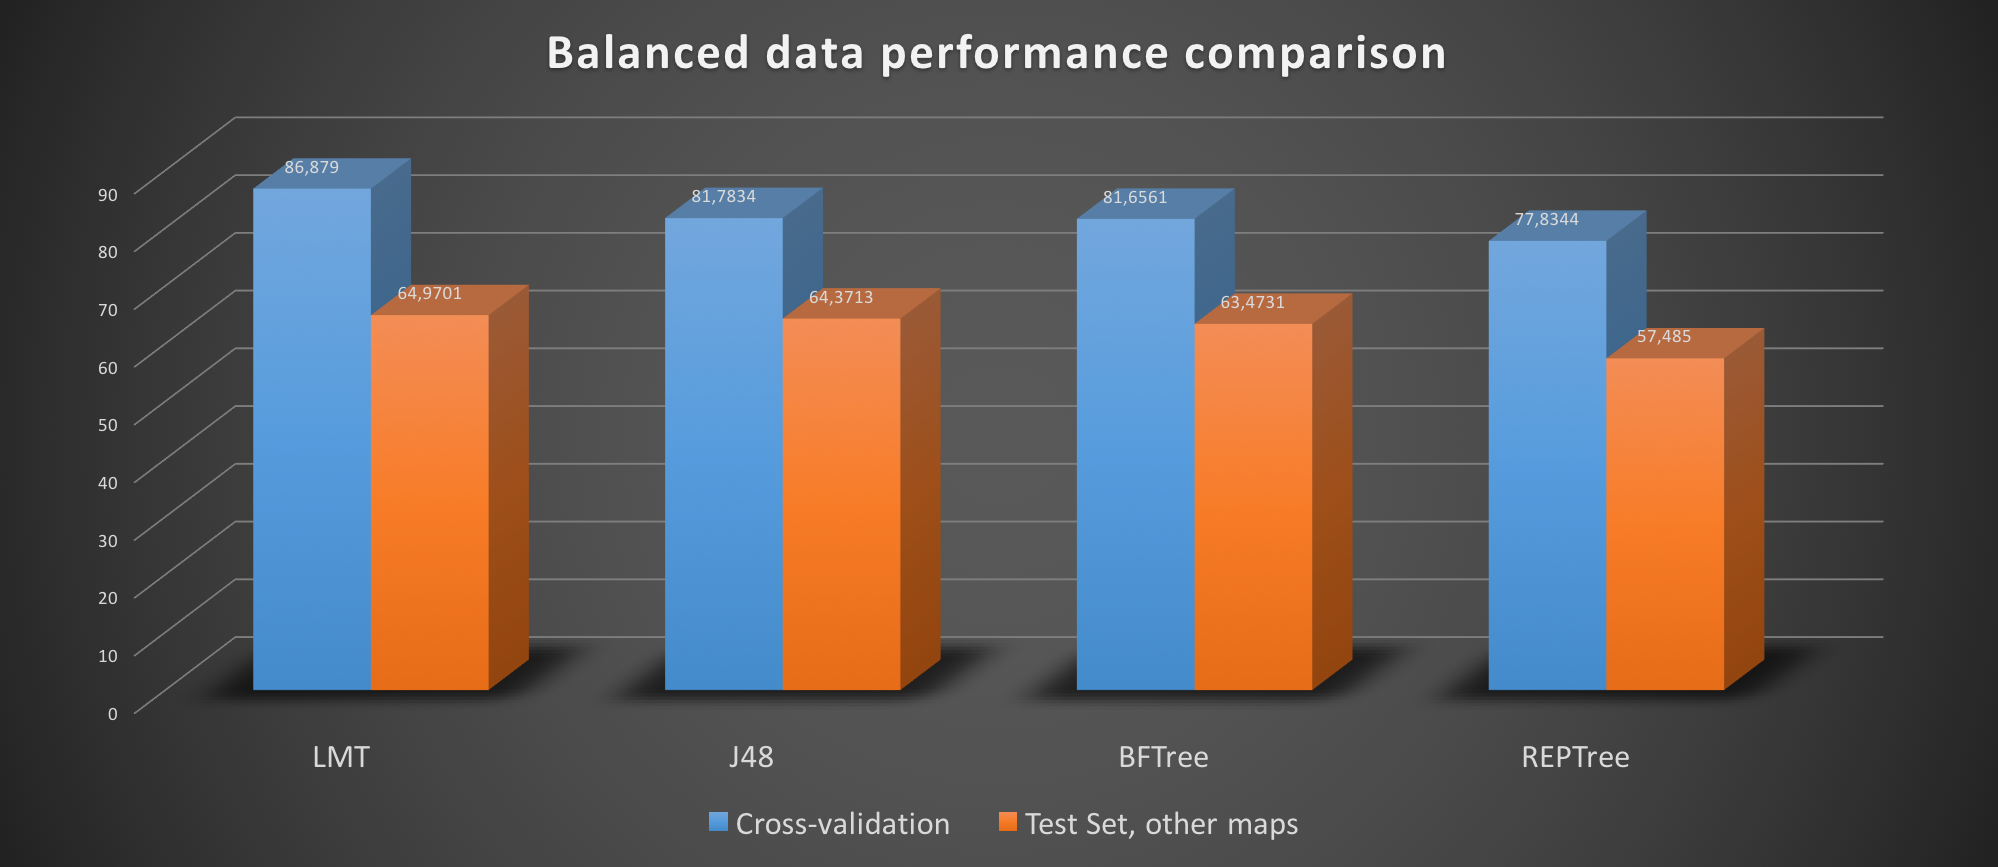
\includegraphics[width=\textwidth]{balanced_performance}

\vspace{0.3cm}

Si bien observamos una clara mejora (de entre el 10 y el 20\%) cuando evaluamos los modelos con validación cruzada, los resultados son desfavorables al evaluar los modelos con una pila de instancias adicional, en otros mapas, decrementando entre un 1 y un 11\% el éxito en clasificación cuando lo comparamos con los datos en bruto.

\subsection{Implementación}

Para la implementación del agente automático teníamos dos opciones: bien escoger uno de los modelos que hemos obtenido previamente con Weka e implementarlo manualmente, o usar un wrapper de \emph{Weka} para \texttt{Python} que, dado un modelo en un fichero \texttt{.model} (o un fichero \texttt{.arff} a partir del cual generarlo), nos devuelva la clase a la que pertenece una instancia dada.

En nuestro caso, decidimos escoger la segunda opción por varios motivos. Primero, porque queríamos experimentar cómo funcionan \texttt{Python} y \emph{Weka} juntos, ya que \emph{Weka} está desarrollada en \texttt{Java}; y segundo porque nos parecía un enfoque mucho más interesante y eficiente, pues de esta forma es más sencillo probar diferentes agentes sin necesidad de reescribir todo el código del agente en cuestión.

Para poder usar \emph{Weka} en \texttt{Python} debemos usar un \href{https://pythonhosted.org/python-weka-wrapper/}{\water{Wrapper}}. Lo primero es seguir los pasos que dan para su instalación, ya que es necesario instalar una serie de librerías para que todo funcione correctamente y, una vez configurado el entorno, debemos abrir nuestro fichero de datos e indicarle a \emph{Weka} cuál de los atributos de este fichero es la clase. Por convención, es común que la clase sea el último atributo de una instancia y, como este es nuestro caso, simplemente llamamos al método \texttt{class\_is\_last()} para indicar que efectivamente nuestra clase está en la última posición de nuestros datos.

Para realizar la clasificación, \emph{Weka} proporciona la clase \texttt{Clasifier}, a la que se le puede indicar qué algoritmo queremos usar. Por ejemplo, si queremos usar \emph{J48}, nuestra creación de la instancia del clasificador deberá ser \texttt{Classifier(classname="weka.classifiers.trees.J48", options=["-C", "0.3"])}. El modelo generado por este clasificador se escribe en un fichero con extensión \texttt{.model}, y podrá ser usado posteriormente para clasificar nuevas instancias. Fue en la parte de uso de dicho modelo es en la que hemos encontrado más dificultades, puesto que \emph{Weka} no está pensado para clasificar instancias en tiempo de ejecución, sino para tratar ficheros de datos \emph{estáticos}, que no van cambiando a medida que se ejecuta un programa.

Nuestra primera idea tras investigar en los ejemplos que hay publicados usando el wrapper, mirar en la documentación y preguntar al profesor fue emplear los métodos \texttt{create\_numeric} y \texttt{create\_nominal} de la clase \texttt{Attribute} para crear e indicar nombre y tipo de los datos de nuestra instancia. Después, se inicializa la instancia con \texttt{Instance.create\_instance} para posteriormente pasársela al clasificador. A este método se le pasa una lista en la que cada posición se corresponde con el valor de un atributo. En principio, tenía mucho sentido que esta implementación funcionase, pero \emph{Weka} por debajo convierte los datos de tipo nominal a \texttt{float} y, en este caso, no era capaz de realizar una conversión o un mapeo de \texttt{string} a \texttt{float}. En este punto, lo siguiente que probamos fue realizar nosotros mismos este \emph{mapeo}, usando un diccionario, pero nuevamente surgían errores que no llegábamos a comprender del todo, así que finalmente cambiamos totalmente el enfoque para solucionar el problema.

En el segundo intento de implementar el clasificador de nuevas instancias, la parte de generar el modelo es exactamente igual que la descrita antes. Sin embargo, probamos una nueva forma de pasar nuestros datos en \emph{raw} a instancias que \emph{Weka} es capaz de comprender. Para ello, escribimos en un archivo las cabeceras de \emph{Weka} que contienen los datos y su tipo, y después escribimos una línea con los datos de nuestra instancia, con la particularidad de que el valor de la clase es una interrogación (?). Esto le indica a \emph{Weka} que no sabemos el valor de la clase. A continuación, cargamos el archivo que acabamos de escribir y obtenemos nuestra instancia gracias al método \texttt{classify\_instance()} de la clase \texttt{Classifier}. Este método devuelve un \texttt{float} ---se ve que esta vez \emph{Weka} sí que es capaz de realizar la conversión de nominal a float...--- que se corresponde con el índice del valor de la clase en su declaración en la cabecera del archivo. Finalmente, devolvemos la dirección correspondiente si está dentro del conjunto de direcciones permitidas, o una de las direcciones adyacentes a esta en su defecto (si el resultado es \emph{North}, pero no está permitida, devolveremos \emph{East} o \emph{West}).

\newpage
\section{Fase 3: Predicción}

Para iniciar esta nueva fase, partimos de los datos que ya seleccionamos en la \emph{Fase 2}, i.e. los datos del agente de teclado, pero esta vez sí podremos utilizar los atributos \texttt{score2} y \texttt{score5} para los predictores de la puntuación dentro de dos y cinco jugadas, respectivamente.

\subsection{Transformación de datos}

Antes de considerar el resto de atributos, queremos razonar sobre la exclusión o inclusión de la clase en el modelo de predicción para puntuaciones futuras. Si bien la inclusión de \texttt{move} seguramente resulte en una mejoría en la regresión, esta será despreciable teniendo en cuenta que sí se está analizando el movimiento anterior (a través del atributo \texttt{direction}) y, por el contrario, implicaría la inutilidad del predictor a la hora de generar el valor para el atributo de la puntuación futura ya que sólo podría generar la predicción después de clasificar la instancia, que es para lo que está pensado. Siguiendo este razonamiento, hemos optado por \textbf{excluir la clase en el predictor}, y así poder utilizarlo en nuestro agente.

Además de este cambio sobre los datos para los dos predictores que vamos a implementar (puntuación para 2 y 5 turnos vista, respectivamente), para cada uno de ellos debemos eliminar también el campo opuesto. Así, para el predictor de $N=2$ eliminaremos \texttt{score5} y viceversa.

\subsection{Experimentación y comparaciones}

Siguiendo la motivación de la \emph{Fase 2}, planteamos distintas alternativas para mejorar el rendimiento de nuestro predictor a la hora de clasificar. Pueden observarse en la siguiente gráfica los resultados de los distintos modelos de regresión generados con \emph{REPTree} en las que se demuestra nuestra hipótesis respecto a la exclusión de \texttt{move}: el empeoramiento en rendimiento del algoritmo es despreciable.

\vspace{0.3cm}

\noindent 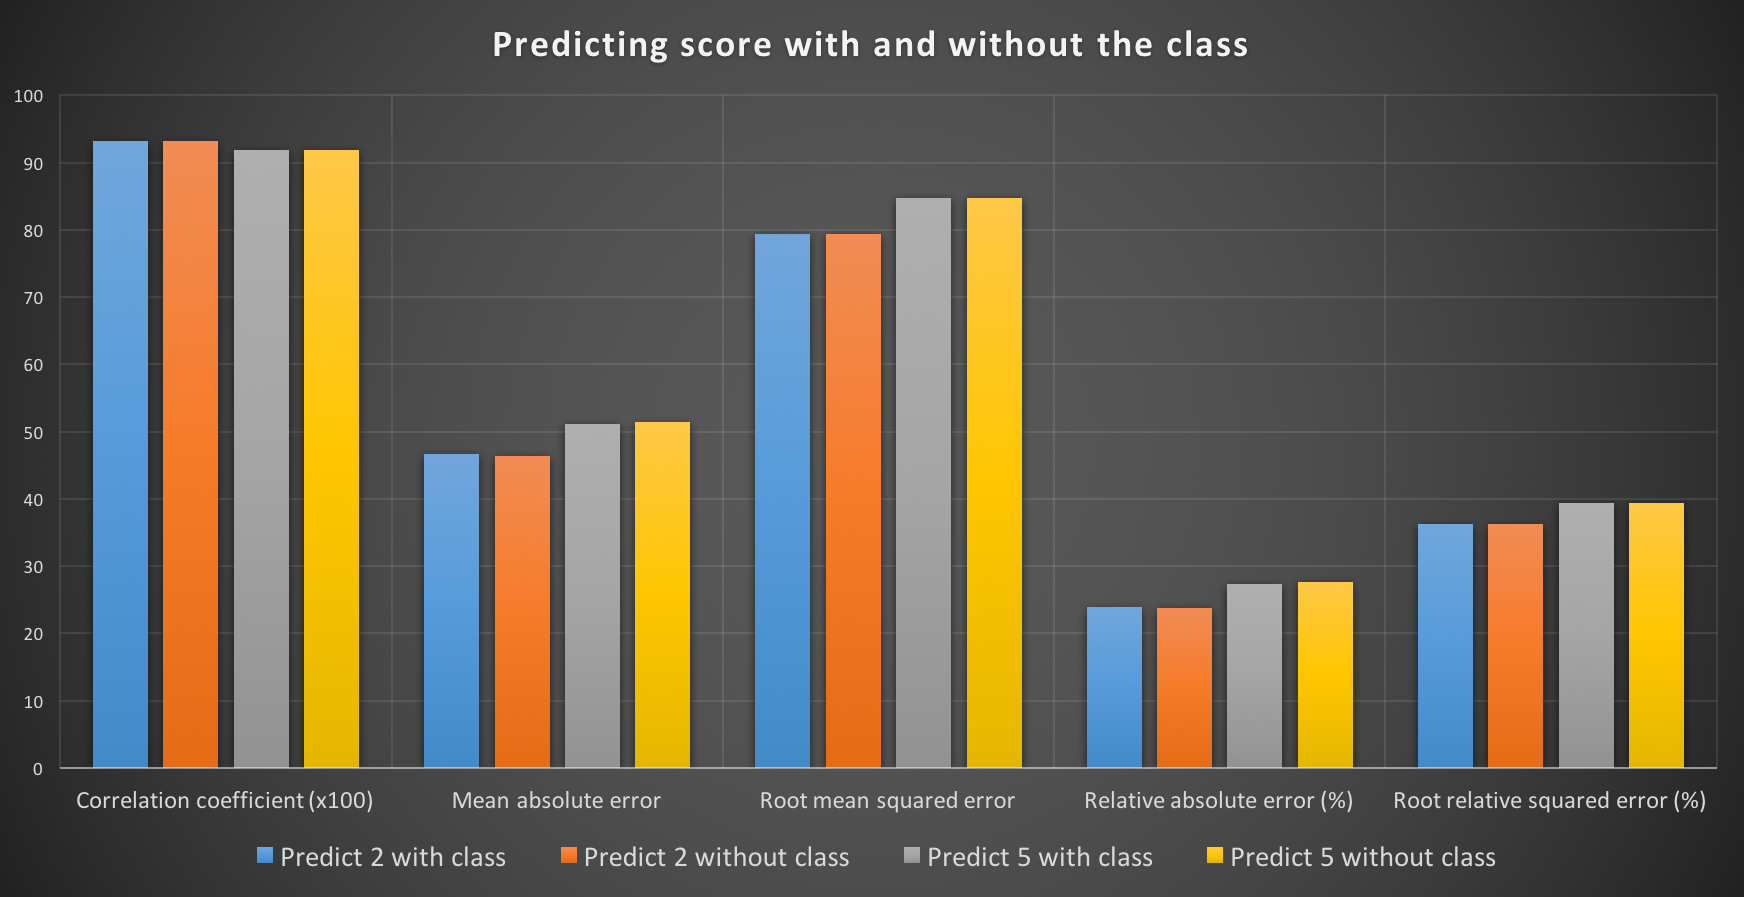
\includegraphics[width=\textwidth]{class_or_no}

\vspace{0.3cm}

No contentos con este hallazgo, procedemos ahora a comparar también el algoritmo que utilizamos en la \emph{Fase 2} con otro nuevo, \emph{M5}. Ya que \emph{REPTree} es el único algoritmo capaz de dar una regresión como resultado de los utilizados en la fase anterior, nos vemos obligados a buscar nuevos algoritmos que comparar. La siguiente gráfica compara sendos generadores de modelos:

\vspace{0.3cm}

\noindent 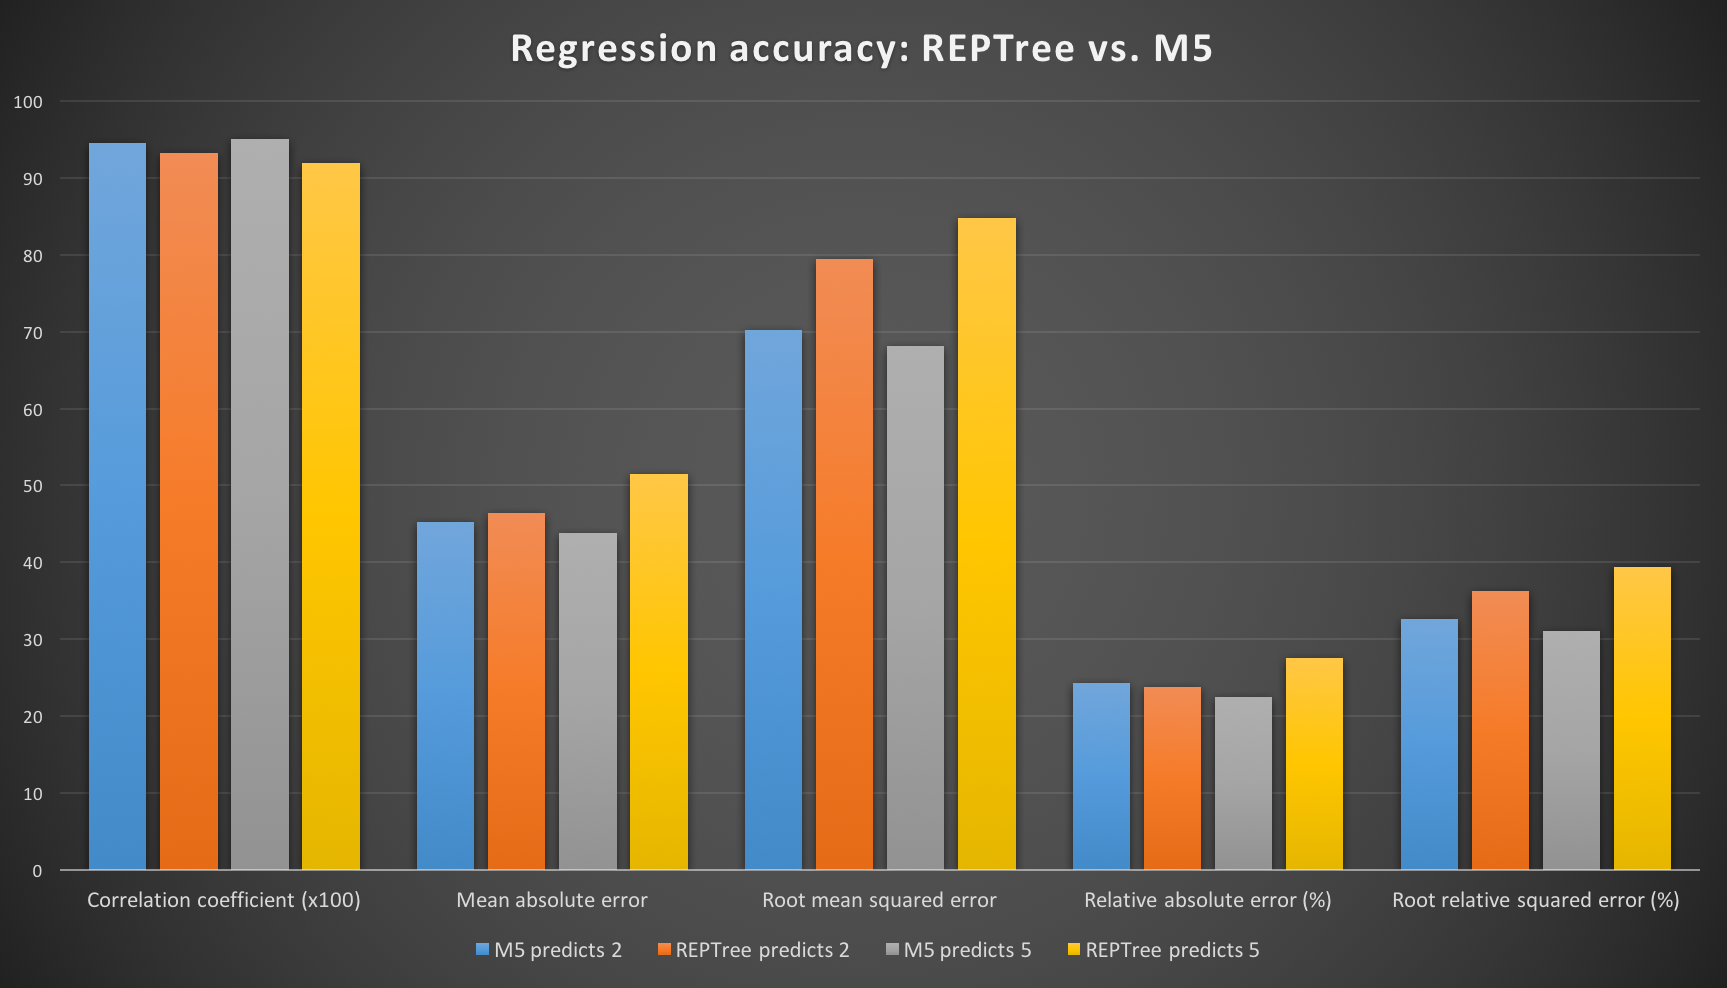
\includegraphics[width=\textwidth]{REPTree_vs_M5}

\vspace{0.3cm}

Observamos que \emph{M5} reduce de forma visible el error en la predicción a la vez que eleva el coeficiente de correlación, y es por ello que será éste el algoritmo que implementaremos a continuación.

\subsection{Implementación}

\newpage
\section{Preguntas}

\begin{center}
    \vspace{0.5cm} \emph{¿Qué diferencias hay a la hora de aprender esos modelos con instancias provenientes de un agente controlado por un humano y uno automático?}
    \vspace{0.5cm}
\end{center}

Lorem ipsum dolor sit amet, consectetur adipisicing elit, sed do eiusmod tempor incididunt ut labore et dolore magna aliqua. Ut enim ad minim veniam, quis nostrud exercitation ullamco laboris nisi ut aliquip ex ea commodo consequat. Duis aute irure dolor in reprehenderit in voluptate velit esse cillum dolore eu fugiat nulla pariatur. Excepteur sint occaecat cupidatat non proident, sunt in culpa qui officia deserunt mollit anim id est laborum.

\begin{center}
    \vspace{0.5cm} \emph{¿Crees que los resultados del modelo de regresión a 5 turnos vista guardan relación con los de 2 turnos? ¿Por qué?}
    \vspace{0.5cm}
\end{center}

Lorem ipsum dolor sit amet, consectetur adipisicing elit, sed do eiusmod tempor incididunt ut labore et dolore magna aliqua. Ut enim ad minim veniam, quis nostrud exercitation ullamco laboris nisi ut aliquip ex ea commodo consequat. Duis aute irure dolor in reprehenderit in voluptate velit esse cillum dolore eu fugiat nulla pariatur. Excepteur sint occaecat cupidatat non proident, sunt in culpa qui officia deserunt mollit anim id est laborum.

\begin{center}
    \vspace{0.5cm} \emph{Si quisieras transformar la tarea de regresión en clasificación ¿Qué tendrías que hacer? ¿Cuál crees que podría ser la aplicación práctica de predecir la puntuación?}
    \vspace{0.5cm}
\end{center}

Lorem ipsum dolor sit amet, consectetur adipisicing elit, sed do eiusmod tempor incididunt ut labore et dolore magna aliqua. Ut enim ad minim veniam, quis nostrud exercitation ullamco laboris nisi ut aliquip ex ea commodo consequat. Duis aute irure dolor in reprehenderit in voluptate velit esse cillum dolore eu fugiat nulla pariatur. Excepteur sint occaecat cupidatat non proident, sunt in culpa qui officia deserunt mollit anim id est laborum.

\begin{center}
    \vspace{0.5cm} \emph{¿Qué ventajas puede aportar predecir la puntuación respecto a la clasificación de la acción? Justifica tu respuesta.}
    \vspace{0.5cm}
\end{center}

Lorem ipsum dolor sit amet, consectetur adipisicing elit, sed do eiusmod tempor incididunt ut labore et dolore magna aliqua. Ut enim ad minim veniam, quis nostrud exercitation ullamco laboris nisi ut aliquip ex ea commodo consequat. Duis aute irure dolor in reprehenderit in voluptate velit esse cillum dolore eu fugiat nulla pariatur. Excepteur sint occaecat cupidatat non proident, sunt in culpa qui officia deserunt mollit anim id est laborum.

\begin{center}
    \vspace{0.5cm} \emph{¿Crees que se podría conseguir alguna mejora en la clasificación incorporando un atributo que indicase si la puntuación en el instante actual ha descendido o ha bajado?}
    \vspace{0.5cm}
\end{center}

Lorem ipsum dolor sit amet, consectetur adipisicing elit, sed do eiusmod tempor incididunt ut labore et dolore magna aliqua. Ut enim ad minim veniam, quis nostrud exercitation ullamco laboris nisi ut aliquip ex ea commodo consequat. Duis aute irure dolor in reprehenderit in voluptate velit esse cillum dolore eu fugiat nulla pariatur. Excepteur sint occaecat cupidatat non proident, sunt in culpa qui officia deserunt mollit anim id est laborum.

\section{Conclusiones}

Conclusiones técnicas sobre la tarea que se ha realizado.
\begin{itemize}
  \item Apreciaciones más generales como: para qué puede ser útil el modelo obtenido, si al realizar la práctica se os han ocurrido otros dominios en que se pueda aplicar aprendizaje automático, etc.
  \item Descripción de los problemas encontrados a la hora de realizar esta práctica.
  \item Comentarios personales. Opinión acerca de la práctica. Dificultades encontradas, críticas, etc.
\end{itemize}

\end{document}
